\documentclass[10pt]{beamer}

\mode<beamer>
{
  \usetheme{default}
  \usecolortheme[rgb={0,0,0.8}]{structure}
  %\setbeamercolor{normal text}{bg=blue!50}
  %\setbeamercolor{normal text}{fg=blue!50}
  % or ...

  %\setbeamercovered{transparent}
  % or whatever (possibly just delete it)
}

\setbeamertemplate{caption}[numbered]

\usepackage[english]{babel}
% or whatever

%\usepackage[latin1]{inputenc}
% or whatever
\usepackage{hyperref}
\usepackage{times}
\usepackage[T1]{fontenc}
% Or whatever. Note that the encoding and the font should match. If T1
% does not look nice, try deleting the line with the fontenc.

%\usepackage{newcent}
%\usefonttheme{structuresmallcapsserif}

\usepackage{amssymb,latexsym,amsmath}
\usepackage{amsthm}
\usepackage{mathtools}
\input xy 
\xyoption{all}
\usepackage[latin1]{inputenc}
\usepackage{color}
\usepackage{xcolor}
\usepackage{tikz}
\usepackage{fontawesome}


\title[Exploring Tools for Interpretable Machine Learning] % (optional, use only with long paper titles)
{Exploring Tools for Interpretable Machine Learning}

%\subtitle

\author[Dr. Juan Orduz] % (optional, use only with lots of authors)
{Dr. Juan Orduz}
% - Give the names in the same order as the appear in the paper.
% - Use the \inst{?} command only if the authors have different
%   affiliation.

\institute[PyData Global 2021] % (optional, but mostly needed)
{}
% - Use the \inst command only if there are several affiliations.
% - Keep it simple, no one is interested in your street address.

\date[PyData Global 2021] % (optional, should be abbreviation of conference name)
{PyData Global 2021}
% - Either use conference name or its abbreviation.
% - Not really informative to the audience, more for people (including
%   yourself) who are reading the slides online

\subject{data science}
% This is only inserted into the PDF information catalog. Can be left
% out.



% If you have a file called "university-logo-filename.xxx", where xxx
% is a graphic format that can be processed by latex or pdflatex,
% resp., then you can add a logo as follows:

\pgfdeclareimage[height=0.8cm]{university-logo}{images/pydata_global_logo.png}
\logo{\pgfuseimage{university-logo}}

% If you wish to uncover everything in a step-wise fashion, uncomment
% the following command:

%\beamerdefaultoverlayspecification{<+->}


\begin{document}

\begin{frame}
  \titlepage
\end{frame}

\begin{frame}{Outline}
\tableofcontents
\end{frame}

\section{Introduction}

\begin{frame}{Introduction}{Aim and Scope of the Talk}
{\bf What?} In this talk we want to test various ways of getting a better understanding on how machine learning (ML) models generate predictions and how features interact with each other. \\

Key components are:
\begin{itemize}
\item Domain knowledge on the problem. 
\item Understanding on the input data.
\item Understanding the logic behind the ML algorithms.
\end{itemize}
\pause
{\bf How?} We are going to work out a concrete example.
\begin{block}{References}
This talk is based on \href{https://juanitorduz.github.io/interpretable_ml/}{my blog post} (\cite{interpretable_ml_orduz_2021}), which itself is based on these two amazing references:
\begin{itemize}
\item \href{https://christophm.github.io/interpretable-ml-book/}{Interpretable Machine Learning, A Guide for Making Black Box Models Explainable by Christoph Molnar} (\cite{molnar2019})
\item \href{https://github.com/PacktPublishing/Interpretable-Machine-Learning-with-Python}{Interpretable Machine Learning with Python by Serg Mas\'is} (\cite{masis2021})
\end{itemize}
\end{block}
{\bf Remark}: Interpretable ML $\neq$ Causality (see \cite{10.2307/j.ctv1c29t27}, \cite{tdd_sl}, \cite{statrethinkingbook} and \cite{molnar2020interpretable})
\end{frame}

\section{Data Set (\cite{molnar2019})}

\begin{frame}{Target Variable -  cnt: Daily Bike Rents}
\begin{center}
  \begin{figure}
    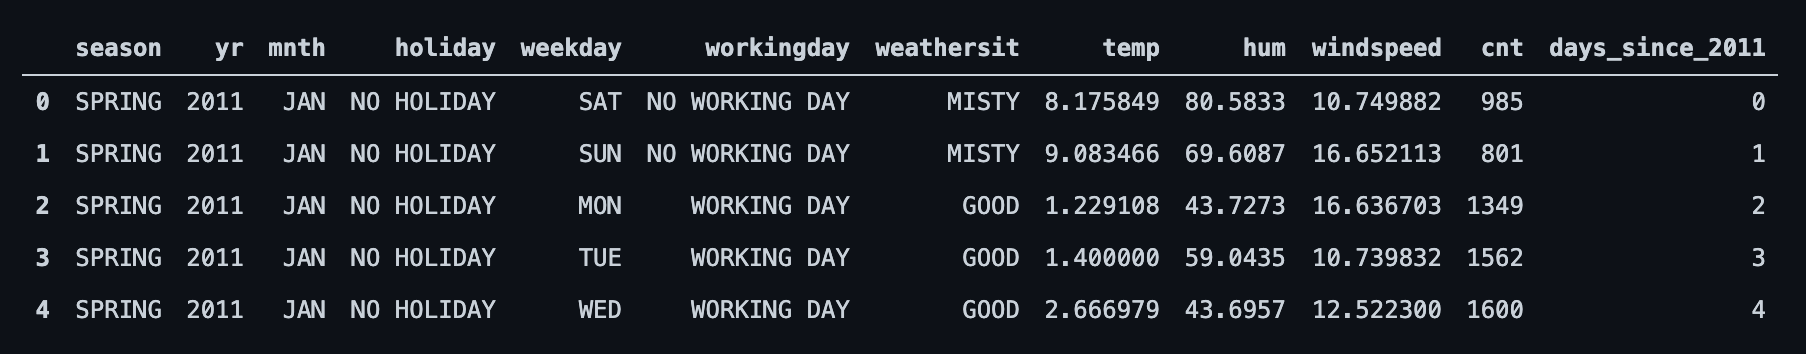
\includegraphics[scale=0.35]{images/head.png} 
    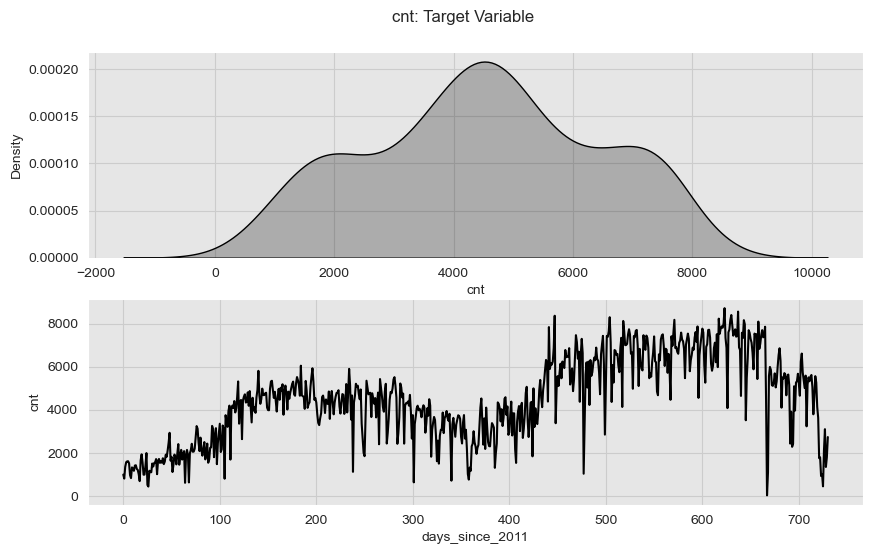
\includegraphics[scale=0.4]{images/interpretable_ml_10_0.png}
  \end{figure}
\end{center}
\end{frame}

\begin{frame}{Continuous Regressors}
\begin{center}
  \begin{figure}
    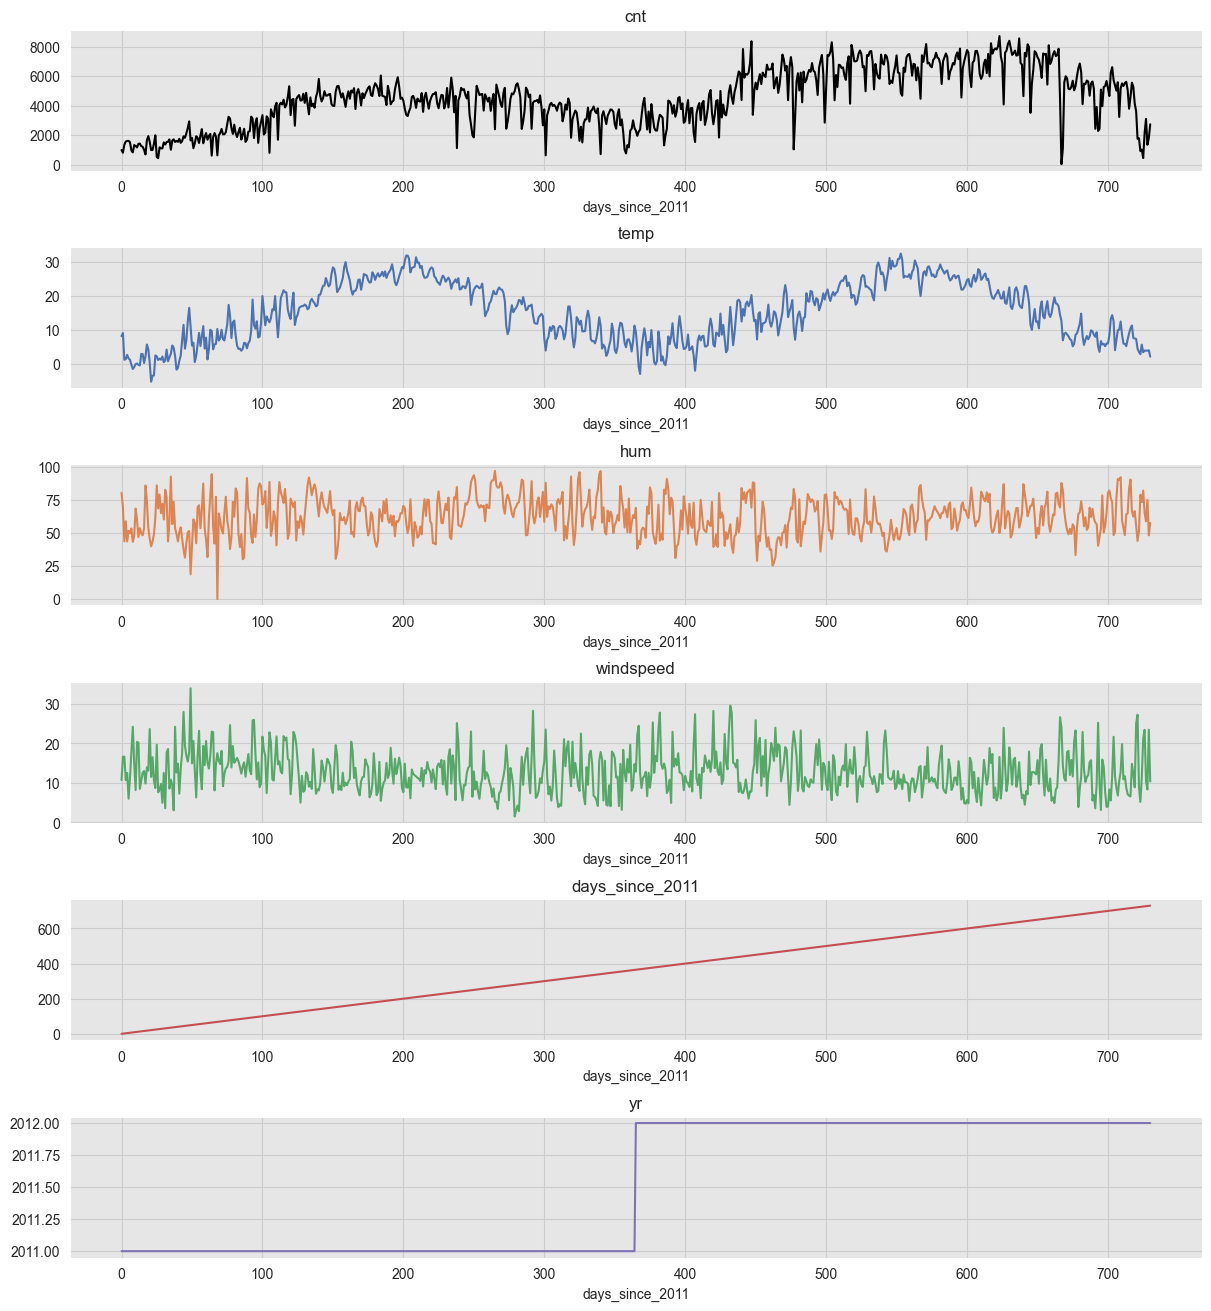
\includegraphics[scale=0.25]{images/interpretable_ml_13_0.png} 
  \end{figure}
\end{center}
\end{frame}

\begin{frame}{Categorical Regressors}
\begin{center}
  \begin{figure}
    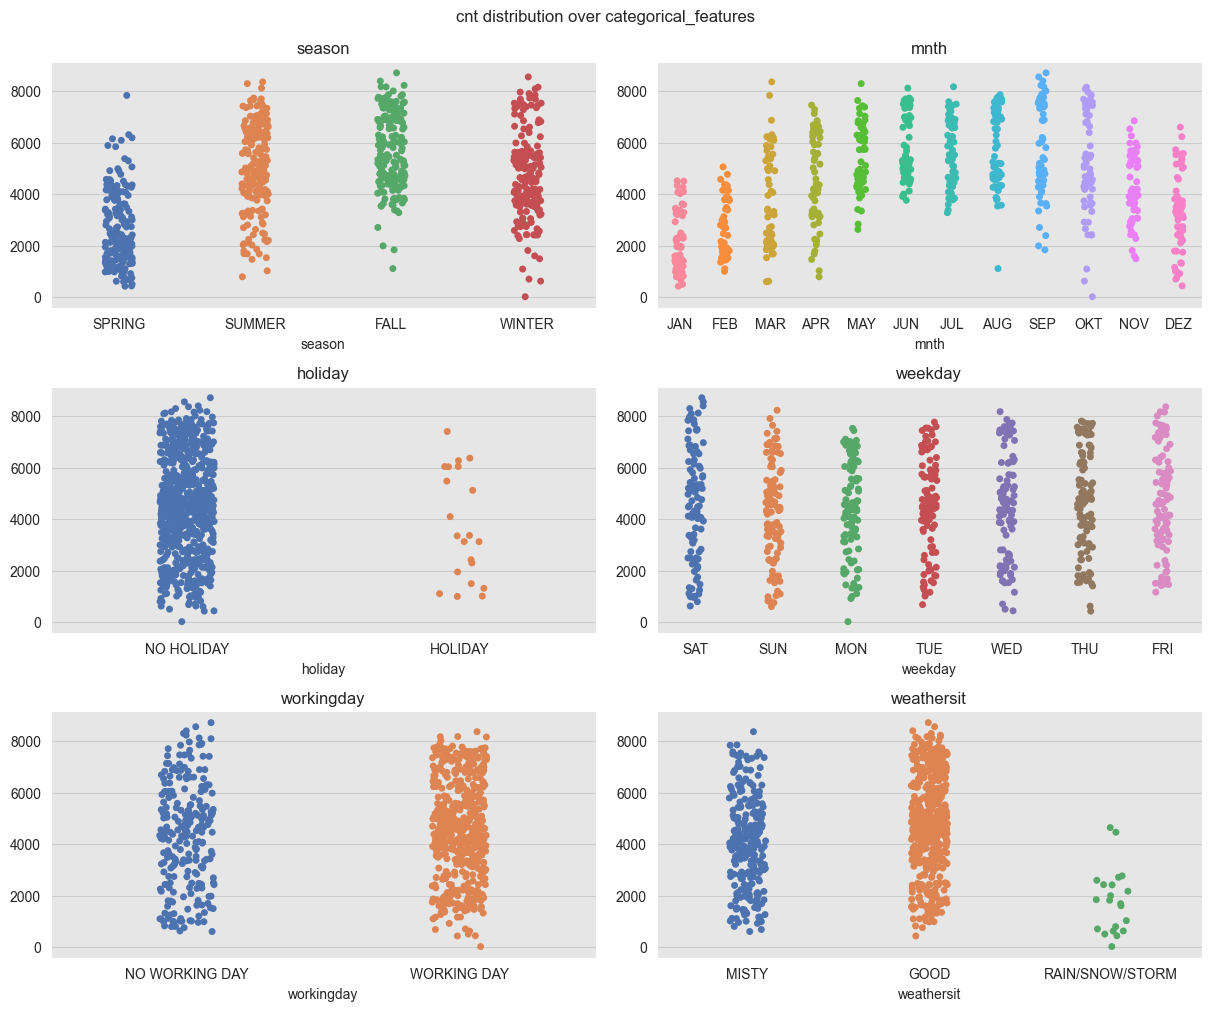
\includegraphics[scale=0.3]{images/interpretable_ml_21_0.png} 
  \end{figure}
\end{center}
\end{frame}

\begin{frame}{Train-Test Split}
\begin{center}
  \begin{figure}
    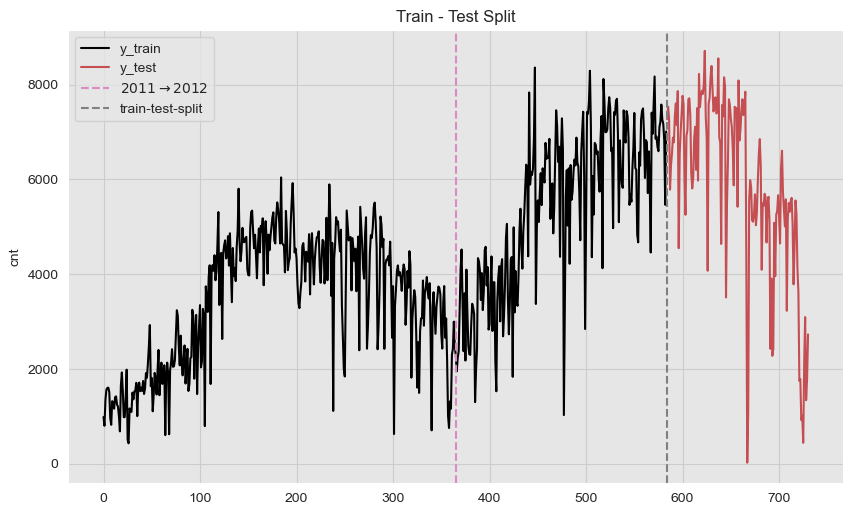
\includegraphics[scale=0.5]{images/interpretable_ml_25_0.png} 
  \end{figure}
\end{center}
\end{frame}

\section{Models Fit (\cite{interpretable_ml_orduz_2021})}

\begin{frame}{Models}{Two model flavours}
\begin{center}
  \begin{figure}
    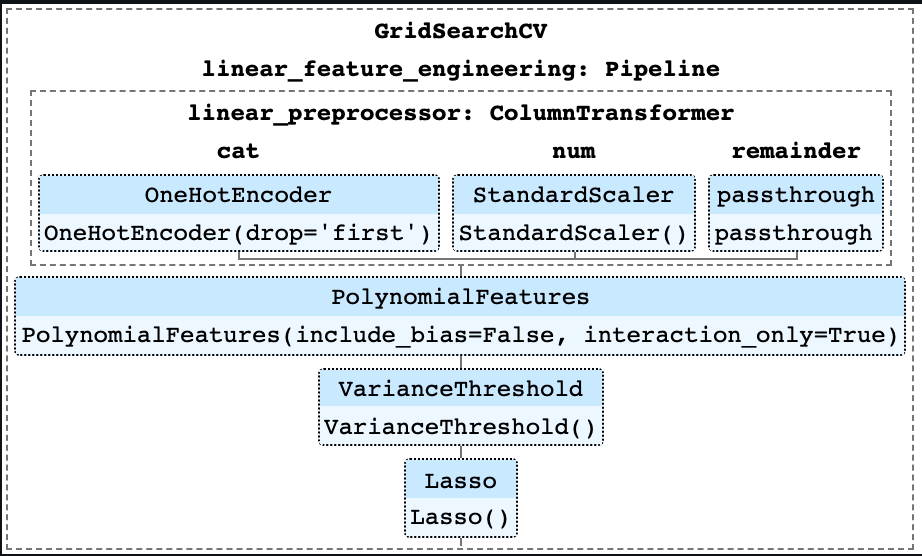
\includegraphics[scale=0.3]{images/linear_grid_search.png}
    \caption{{\bf Linear model} Lasso + second order polynomial interactions (\cite{scikit-learn}).}
  \end{figure}
\end{center}
\begin{center}
  \begin{figure}
    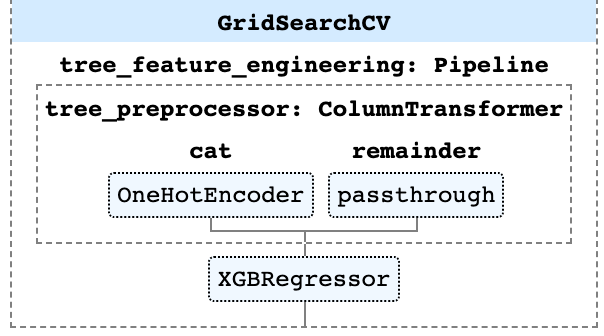
\includegraphics[scale=0.3]{images/tree_grid_search.png}
    \caption{{\bf Tree based model} XGBoost regression model (\cite{xgboost}).}
  \end{figure}
\end{center}
\end{frame}

\begin{frame}{Out of sample performance - Errors Distribution}
\begin{center}
  \begin{figure}
    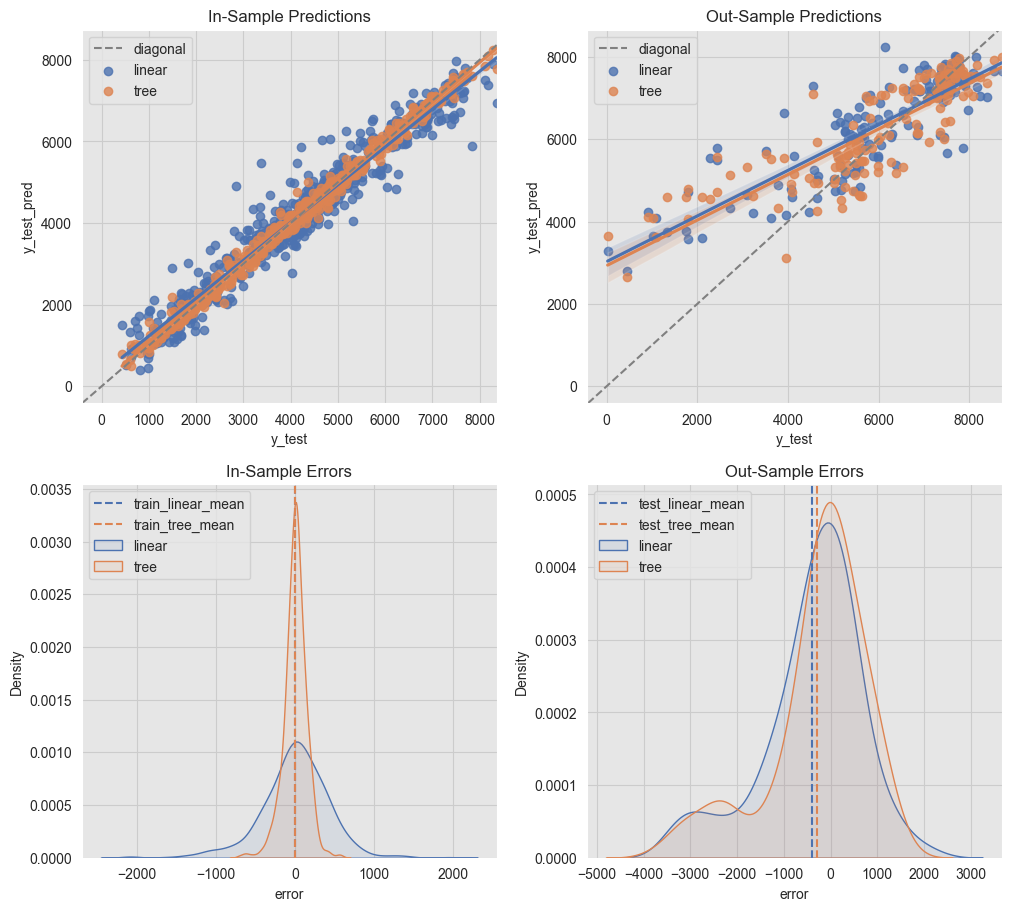
\includegraphics[scale=0.35]{images/interpretable_ml_44_0.png} 
  \end{figure}
\end{center}
\end{frame}

\begin{frame}{Out of sample performance - Predictions}
\begin{center}
  \begin{figure}
    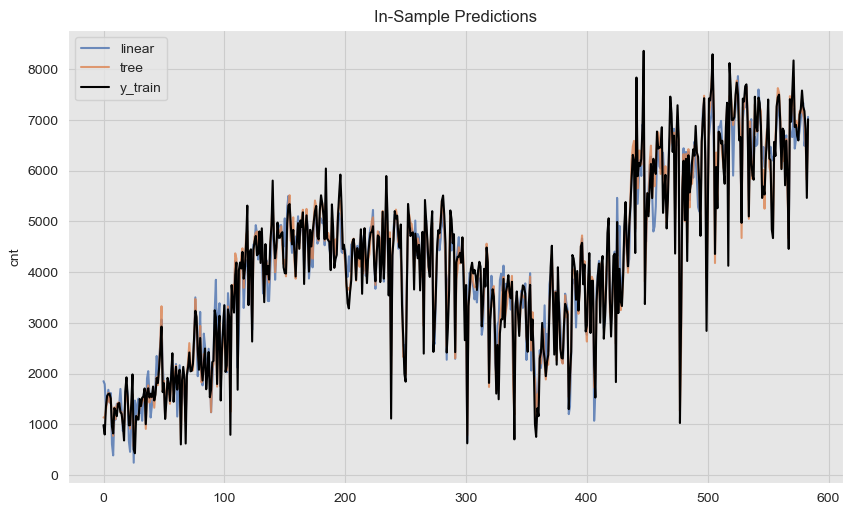
\includegraphics[scale=0.45]{images/interpretable_ml_47_0.png} 
  \end{figure}
\end{center}
\end{frame}

\section{Model Explainability (\cite{molnar2019}, \cite{masis2021})}

\subsection{Model Specific} 

\subsubsection{Beta Coefficients and Weight Effects}

\begin{frame}{$\beta$ coefficients}{See \cite[Section 5.1]{molnar2019}}
\begin{align*}
y = \beta_{0} + \beta_{1}x_{1} + \cdots + \beta_{p}x_{p} + \varepsilon, \quad \text{where} \quad \varepsilon \sim N(0, \sigma^2)
\end{align*}
\begin{center}
  \begin{figure}
    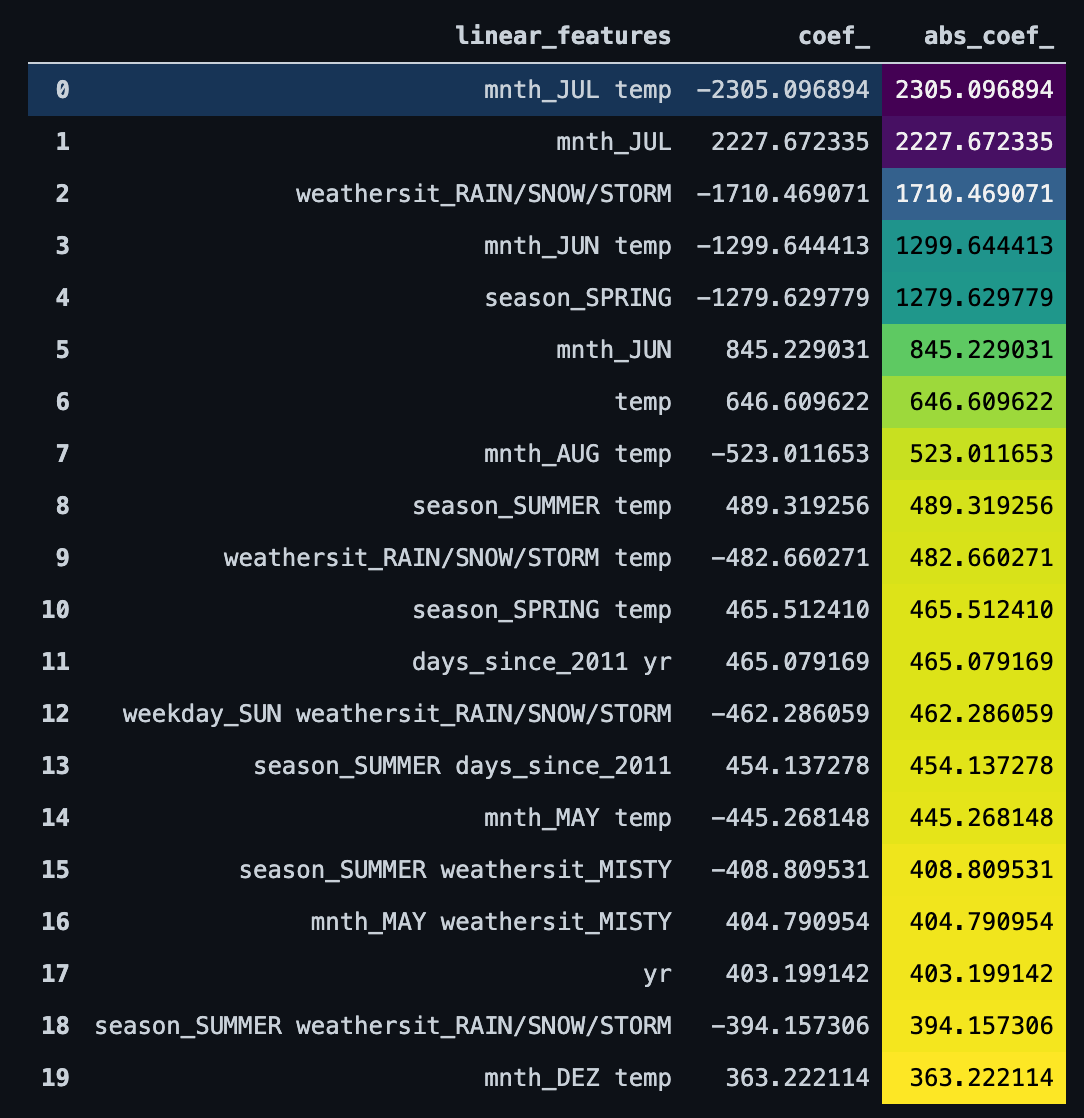
\includegraphics[scale=0.3]{images/lm_beta_table.png} 
  \end{figure}
\end{center}
\end{frame}

\begin{frame}{Weight Effects $\beta_{i}x_{i}$}
\begin{center}
  \begin{figure}
    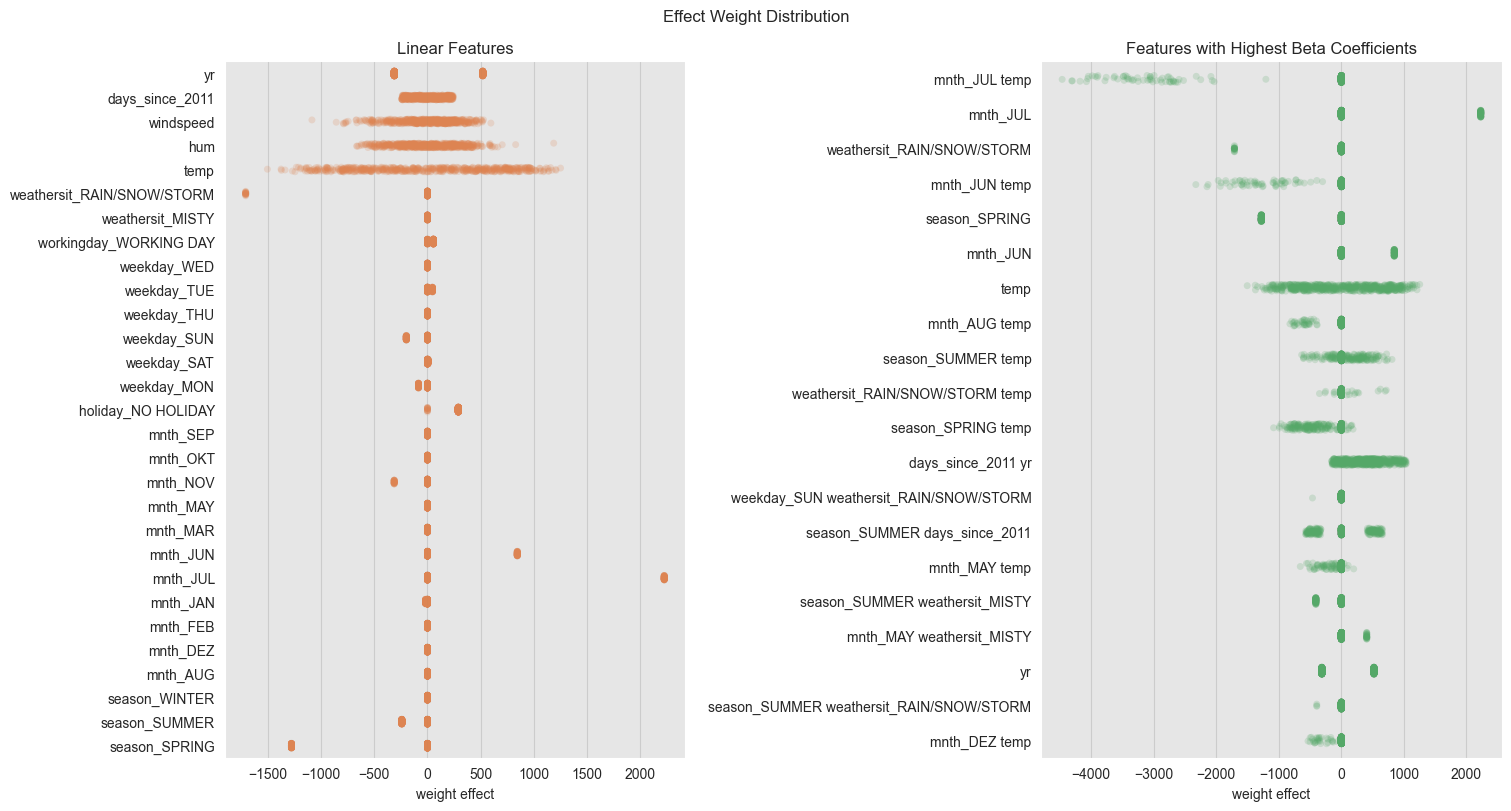
\includegraphics[scale=0.3]{images/interpretable_ml_61_0.png}
    \caption{For each data instance $i$ and each feature $x_{k}$ we compute the product $\beta_{k}x^{(i)}_{k}$ to get the weight effect.}
  \end{figure}
\end{center}
\end{frame}

\begin{frame}{Weight Effects Importance $w_{i} = \frac{1}{n}\sum_{i=1}^{n}|\beta_{i}x_{i}|$}
\begin{center}
  \begin{figure}
    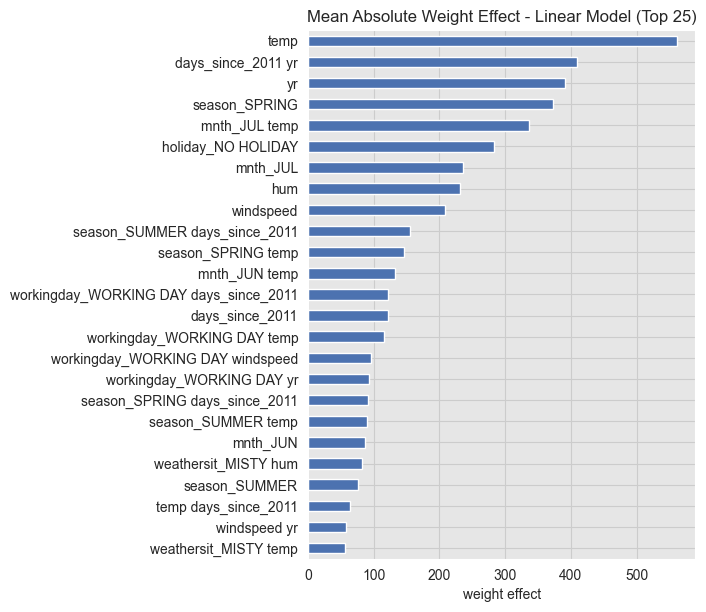
\includegraphics[scale=0.45]{images/interpretable_ml_62_0.png}
  \end{figure}
\end{center}
\end{frame}

\begin{frame}{Weight Effects: Temperature (z-transform)}
\begin{center}
  \begin{figure}
    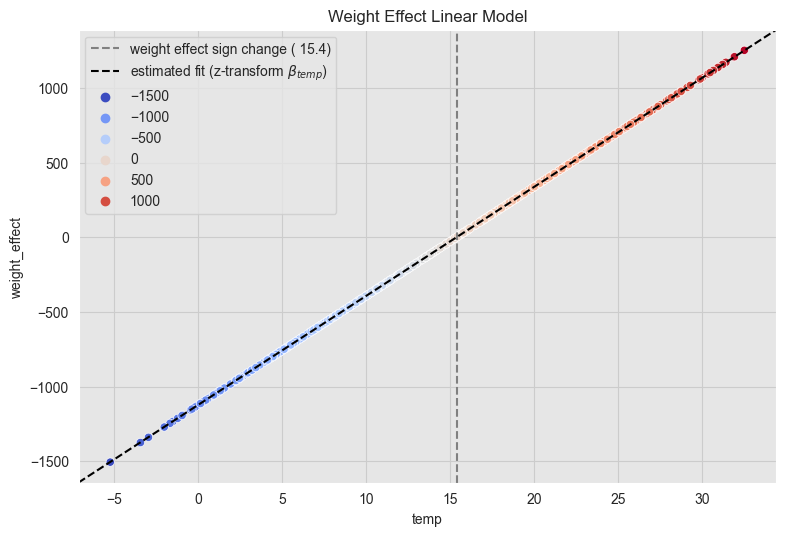
\includegraphics[scale=0.48]{images/interpretable_ml_65_0.png}
    \caption{This plot just shows the effect of the linear term {\em temp} and not the interactions.}
  \end{figure}
\end{center}
\end{frame}

\begin{frame}{Weight Effects: Interactions}
\begin{center}
  \begin{figure}
    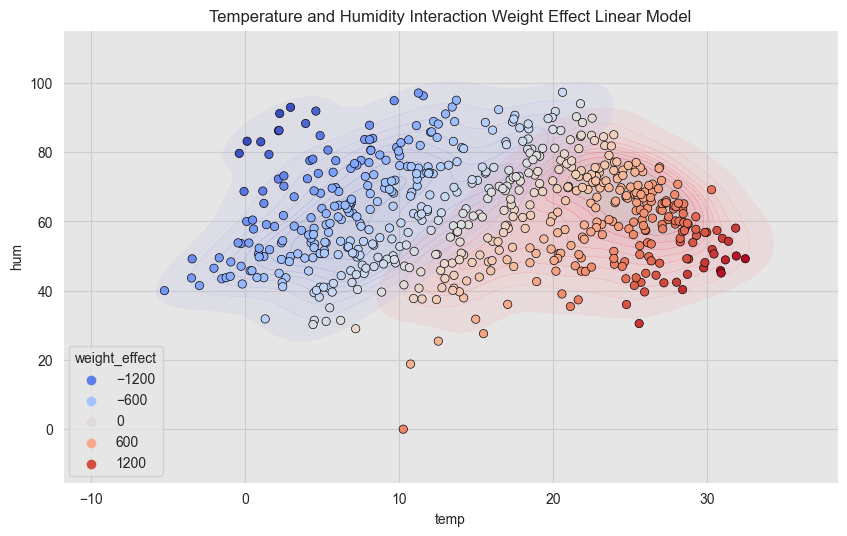
\includegraphics[scale=0.48]{images/interpretable_ml_68_0.png}
    \caption{
      We can visualize the interaction between {\em temp} and {\em hum} by computing the total weight effect $\beta_{temp}x_{temp} + \beta_{hum}x_{hum} + \beta_{temp \times hum}x_{temp}x_{hum}$.
    }
  \end{figure}
\end{center}
\end{frame}

\begin{frame}{Explaining Individual Predictions}{Let us see weight effects of the linear model for data observation 284}
\begin{center}
  \begin{figure}
    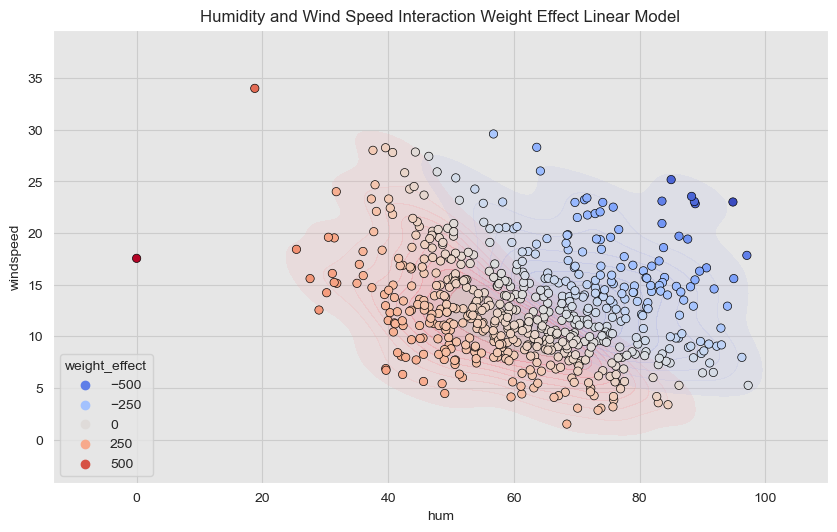
\includegraphics[scale=0.3]{images/interpretable_ml_72_0.png}
    \caption{Left: All weight effects. Right: Weight effects of the linear terms.}\label{fig:linear-284-obs}
  \end{figure}
\end{center}
\end{frame}

\subsubsection{Tree ensembles}

\begin{frame}{Feature Importance Metrics: XGBoost (\cite{xgboost})}

\begin{columns}
\begin{column}{0.4\textwidth}
  \begin{itemize}
  \item {\bf Gain:} improvement in accuracy brought by a feature to the branches it is on.
  \item {\bf Cover:} measures the relative quantity of observations concerned by a feature.
  \item {\bf Frequency / Weight:} just counts the number of times a feature is used in all generated trees.
  \end{itemize}
\end{column}
\begin{column}{0.6\textwidth}
\begin{center}
  \begin{figure}
    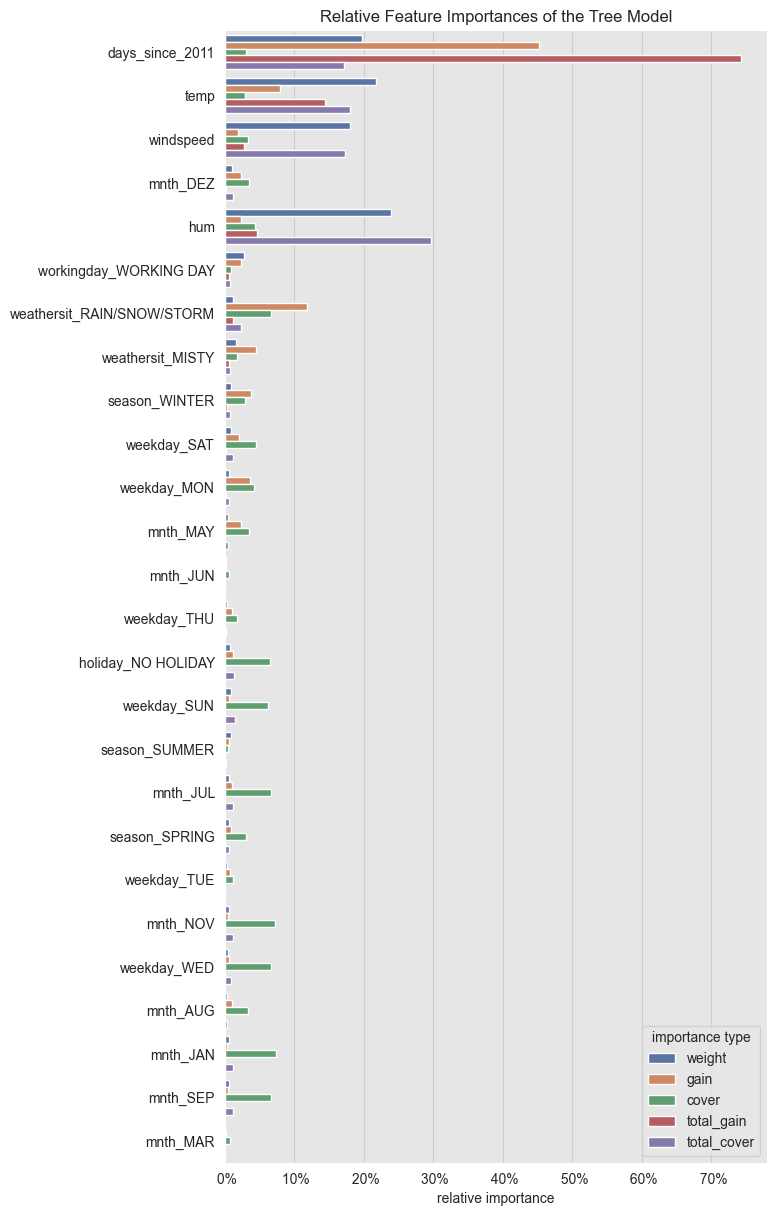
\includegraphics[scale=0.25]{images/interpretable_ml_81_0.png}
  \end{figure}
\end{center}
\end{column}
\end{columns}
\end{frame}

\subsection{Model Agnostic}

\subsubsection{PDP and ICE Plots}

\begin{frame}{Partial Dependence Plot (PDP) \& Individual Conditional Expectation (ICE) (\cite[Section 8.1 \& 9.1]{molnar2019})}
\begin{itemize}
\item The partial dependence plot shows the marginal effect one or two features have on the predicted outcome of a machine learning model. 
\item For example, given a trained model $\hat{f}$, we compute for $\textcolor{red}{temp=8}$
\begin{align*}
\hat{f}_{temp}(\textcolor{red}{temp=8}) = 
\frac{1}{146}
& \left(\hat{f}(\textcolor{red}{temp=8}, hum=80, \cdots) \right.\\
& \left. + \hat{f}(\textcolor{red}{temp=8}, hum=70, \cdots)  + \cdots \right)
\end{align*}
\pause
\item Individual conditional expectation (ICE) plot shows one line per instance. 
\item A PDP is the average of the lines of an ICE plot
\end{itemize}
\end{frame}

\begin{frame}{PDP \& ICE Examples (1D)}
\begin{center}
  \begin{figure}
    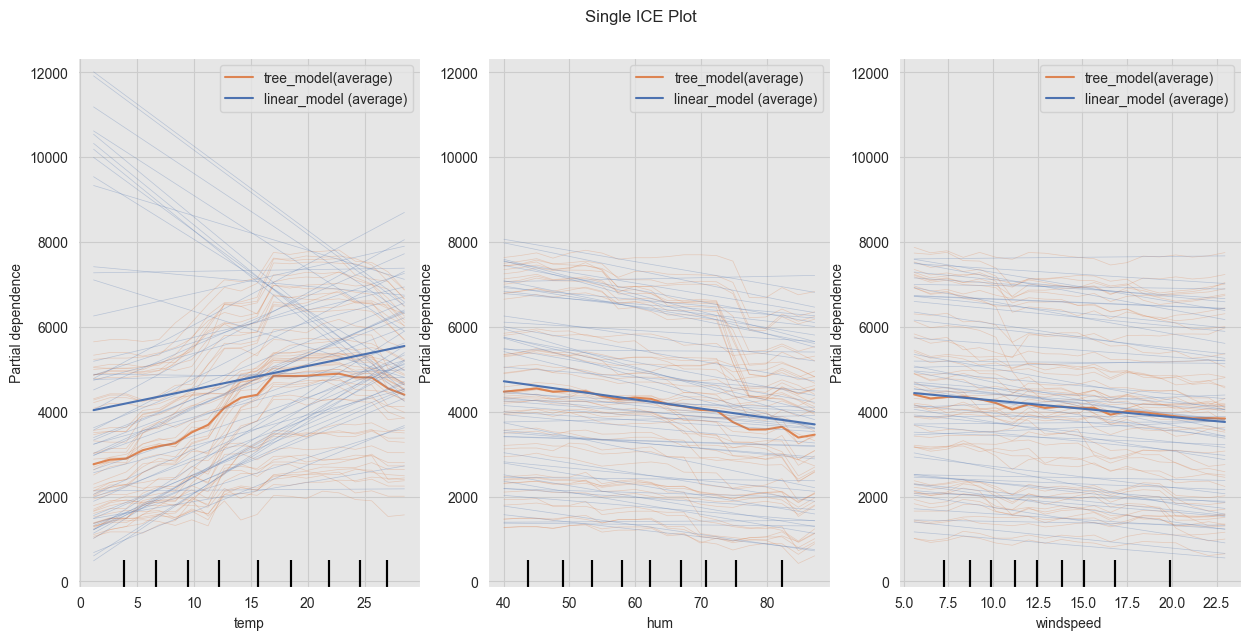
\includegraphics[scale=0.35]{images/interpretable_ml_99_0.png}
    \caption{PDP \& ICE plots for some numerical variables for the linear and XGBoost models.}\label{fig:pdp-ice}
  \end{figure}
\end{center}
\end{frame}

\begin{frame}{PDP \& ICE Examples (2D)}
\begin{center}
  \begin{figure}
    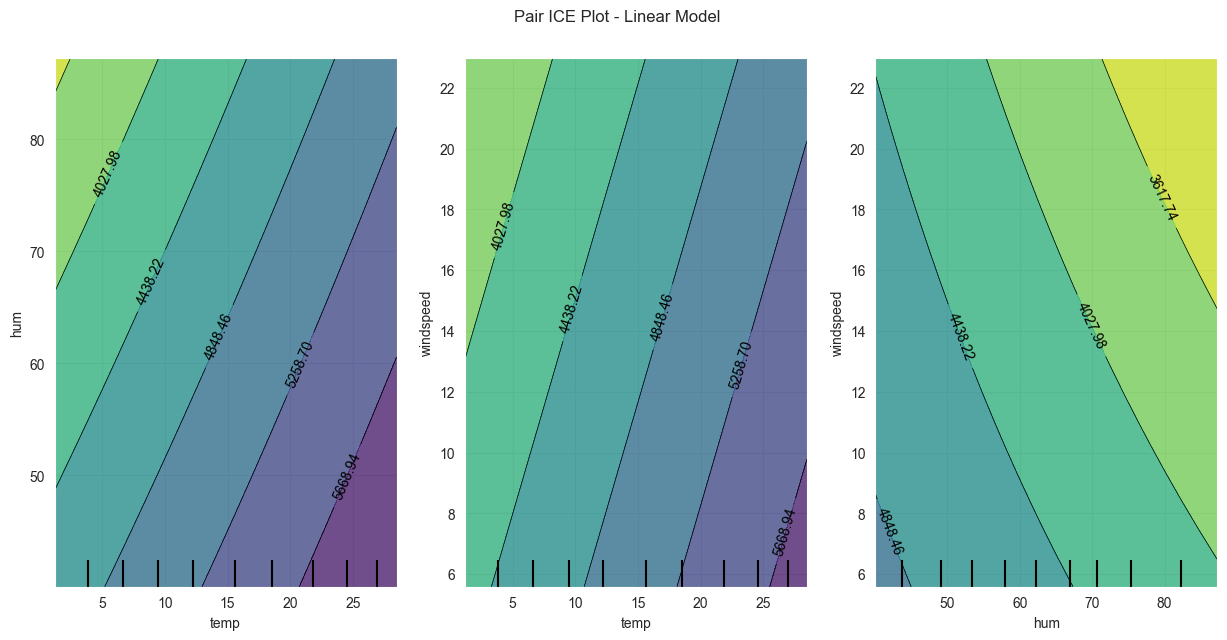
\includegraphics[scale=0.35]{images/interpretable_ml_87_0.png}
    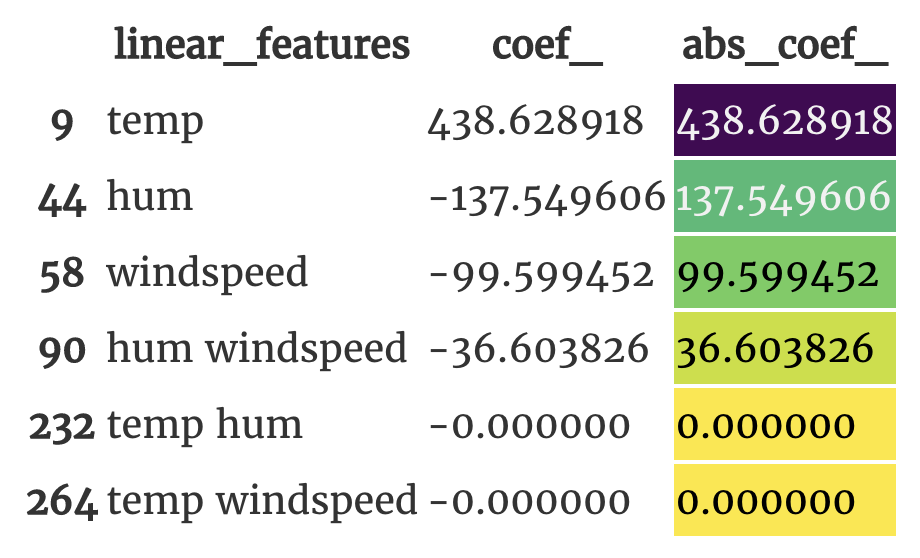
\includegraphics[scale=0.3]{images/interaction_coef.png}
  \end{figure}
\end{center}
\end{frame}


\subsubsection{Permutation Importance}

\begin{frame}{Permutation Importance}{See \cite[Section 5.1]{molnar2019}}
Measures the increase in the prediction error of the model after we permuted the feature's values, which breaks the relationship between the feature and the true outcome (\cite[Section 8.5]{molnar2019}).
\begin{center}
  \begin{figure}
    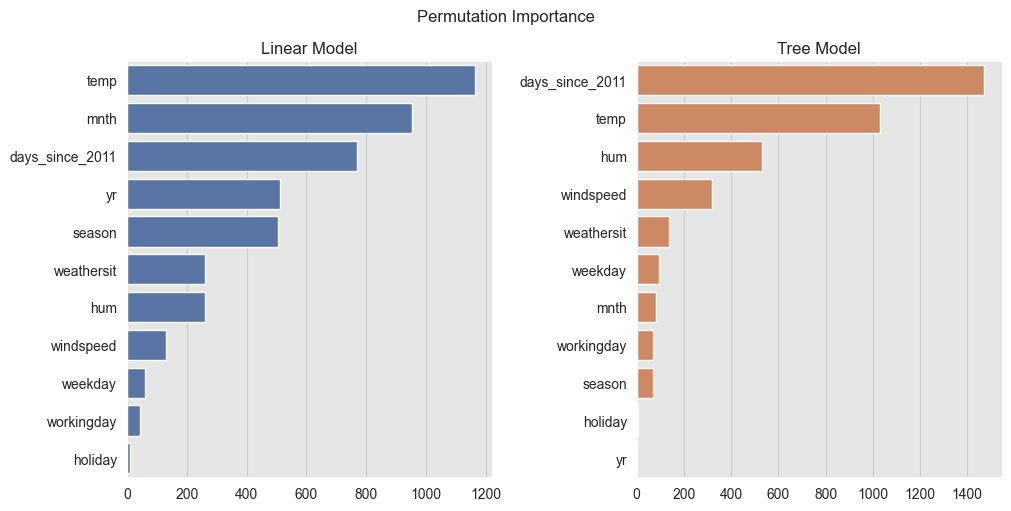
\includegraphics[scale=0.35]{images/interpretable_ml_104_0.png}
    \caption{The permutation importance for these two models have {\em days\_since\_2011} and {\em temp} on their top 3 ranking, which partially explain the trend and seasonality components respectively (see \cite[Figure 8.27]{molnar2019}).}
  \end{figure}
\end{center}
\end{frame}

\subsubsection{SHAP}

\begin{frame}{SHAP Values: Features as teams playing a game}{Definition, see \cite{NIPS2017_7062}, and \cite[Chapters 5 \& 6]{masis2021} and \cite[Section 9.6]{molnar2019}}
For each data instance $x$ (e.g. \textcolor{blue}{temp=15, hum=60, windspeed=14})
\begin{itemize}
\item Sample coalitions $z'\in\{0, 1\}^{M}$, where $M$ is the maximum coalition size.
\begin{itemize}
\item \color{blue} Assume we select $temp$ and $hum$ from $\{temp, hum, windspeed\}$.
\end{itemize}
\pause
\item Get prediction for each $z'$. For features not in the coalition we replace their values with random samples from the dataset (background data).
\begin{itemize}
\item \color{blue} E.g. for a data instance $temp = 15$ and $hum = 60$ we compute the prediction $\hat{f}(temp=15, hum=60, \textcolor{red}{windspeed=11})$.
\end{itemize}
\pause
\item Compute the weight for each $z_{k}'$, with the SHAP kernel, 
$$\pi_{x}(z') = \frac{(M-1)}{\binom{M}{|z'|}|z'|(M-|z'|)} $$
\begin{itemize}
\item \color{blue} $M=3, |z`|=2 \Rightarrow \pi = (3 - 1)/(3 \times 2\times(3 - 2)) = 1/3.$
\end{itemize}
\pause
\item Fit weighted linear model and  return Shapley values, i.e. the coefficients from the linear model.
\end{itemize}
\end{frame}

\begin{frame}{SHAP Values}
\begin{center}
  \begin{figure}
    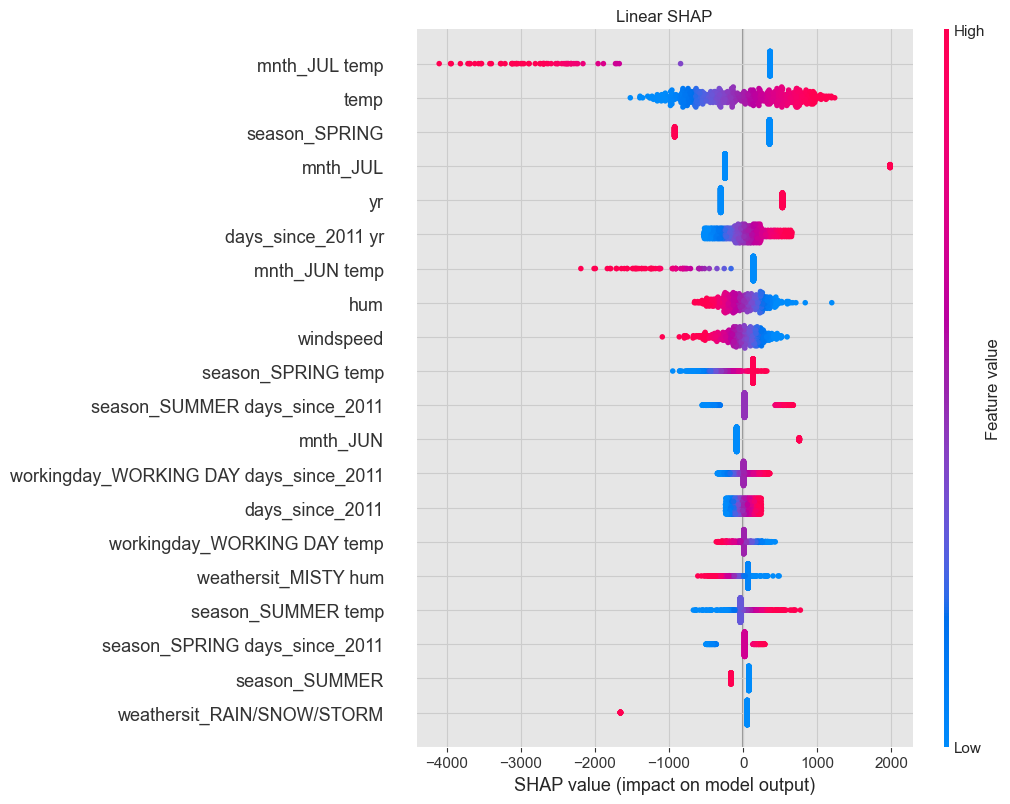
\includegraphics[scale=0.22]{images/interpretable_ml_114_0.png}
    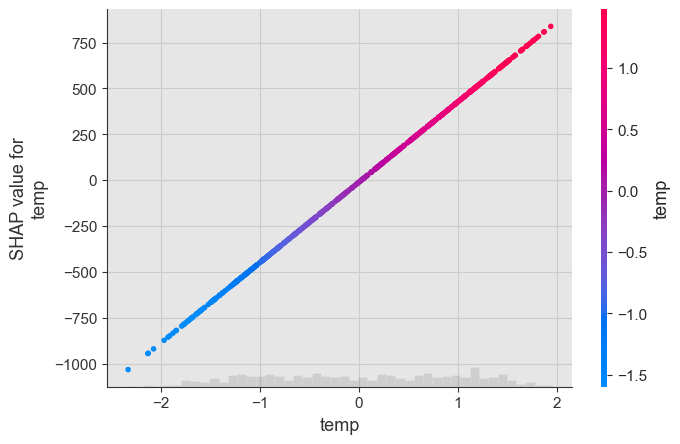
\includegraphics[scale=0.22]{images/interpretable_ml_127_0.png}
    \caption{SHAP values per data instance. The $x$ position of the dot is determined by the SHAP value of that feature, and dots "pile up" along each feature row to show density. Color is used to display the original value of a feature (\cite{NIPS2017_7062}).}
  \end{figure}
\end{center}
\end{frame}

\begin{frame}{Mean Abs SHAP Values}
\begin{center}
  \begin{figure}
    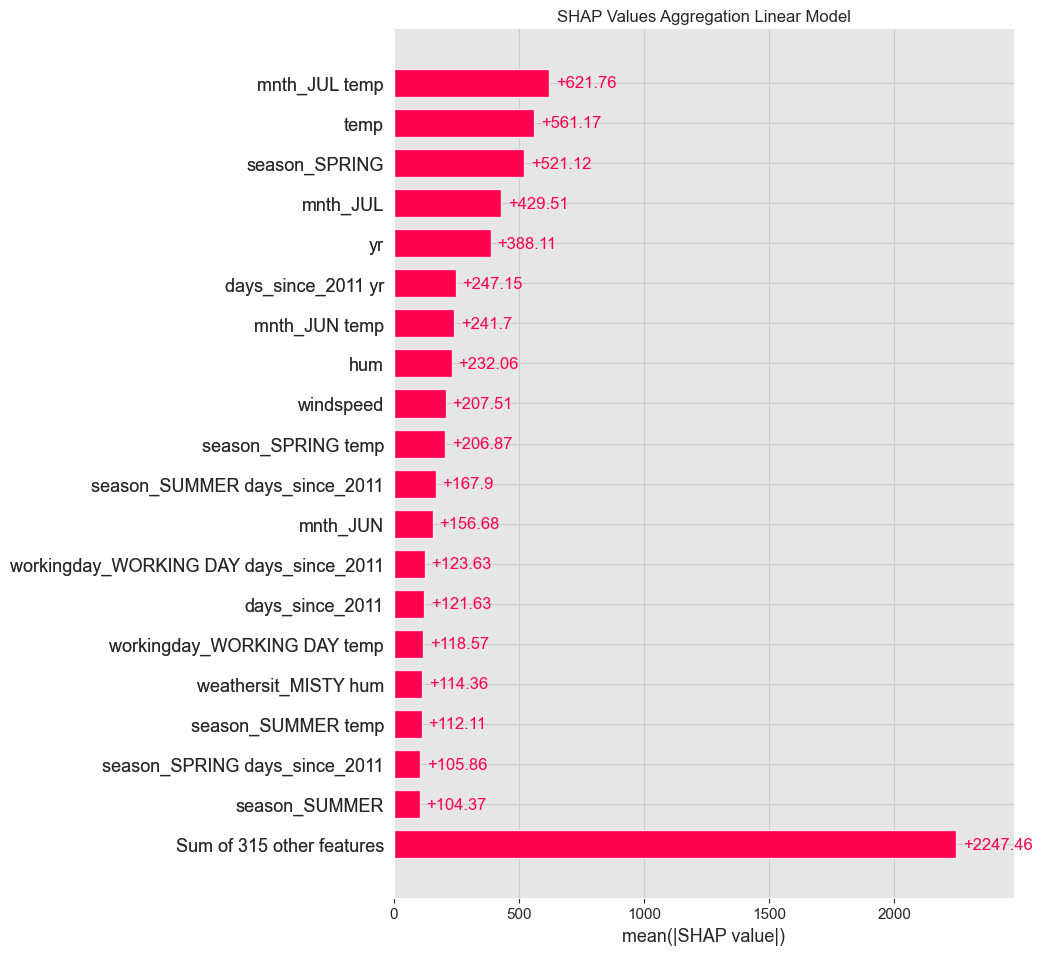
\includegraphics[scale=0.21]{images/interpretable_ml_116_0.png}
    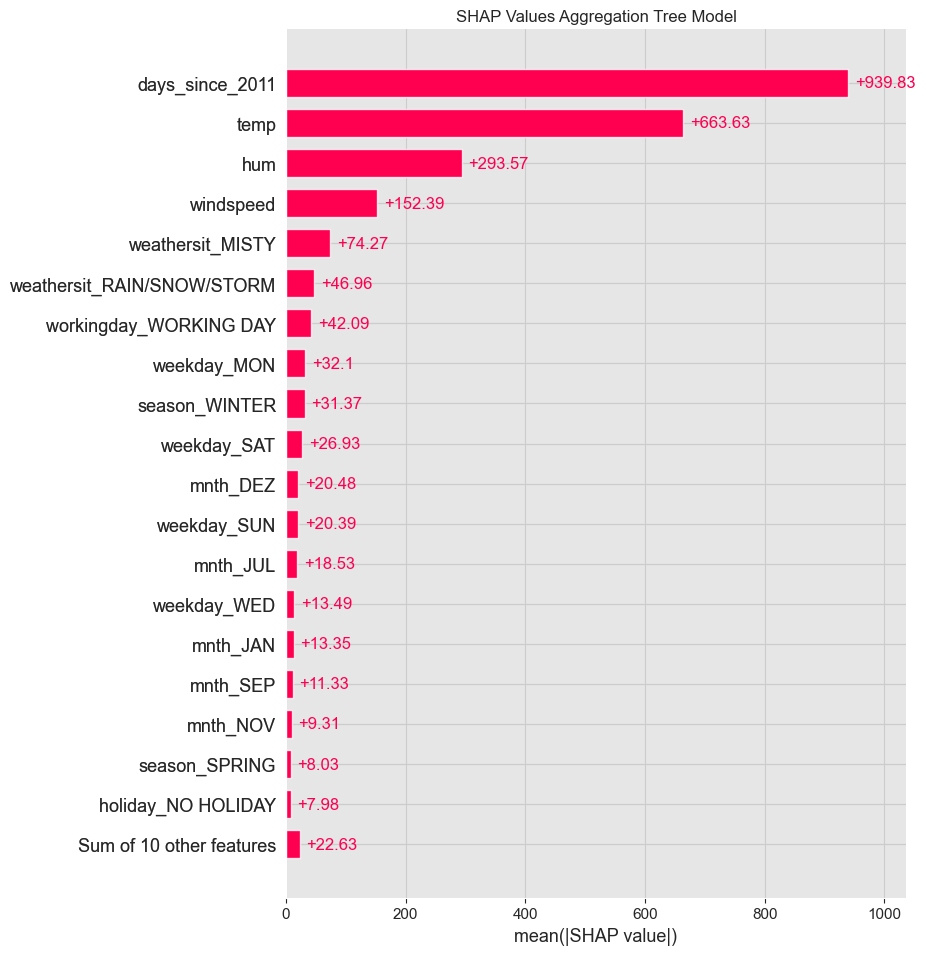
\includegraphics[scale=0.21]{images/interpretable_ml_128_0.png}
  \end{figure}
\end{center}
\end{frame}

\begin{frame}{SHAP Values: Temperature}
\begin{center}
  \begin{figure}
    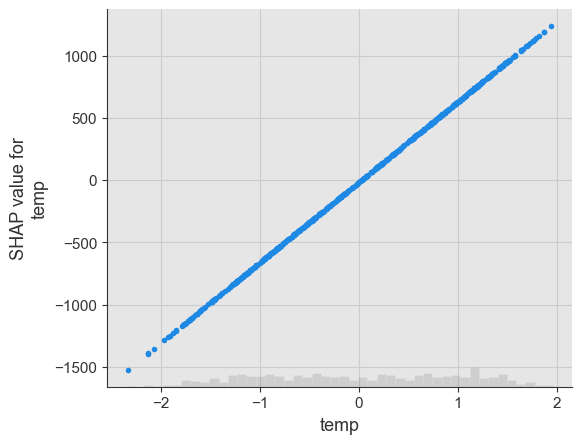
\includegraphics[scale=0.33]{images/interpretable_ml_119_0.png}
    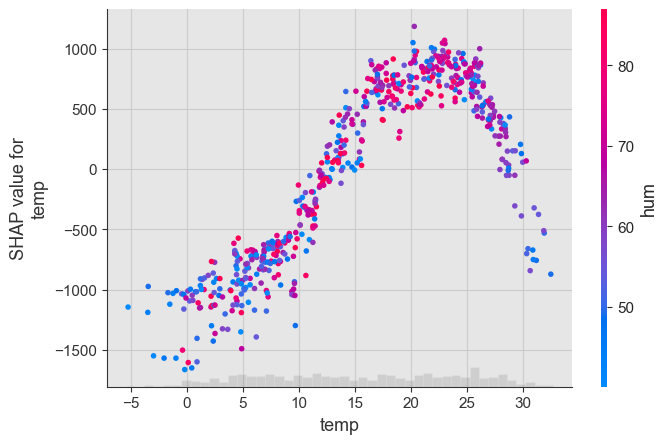
\includegraphics[scale=0.33]{images/interpretable_ml_131_0.png}
    \caption{This figure shows the SHAP values as a function of temperature. Compare with Figure \ref{fig:pdp-ice}}
  \end{figure}
\end{center}
\end{frame}

\begin{frame}{SHAP Values: Observation 284}
\begin{center}
  \begin{figure}
    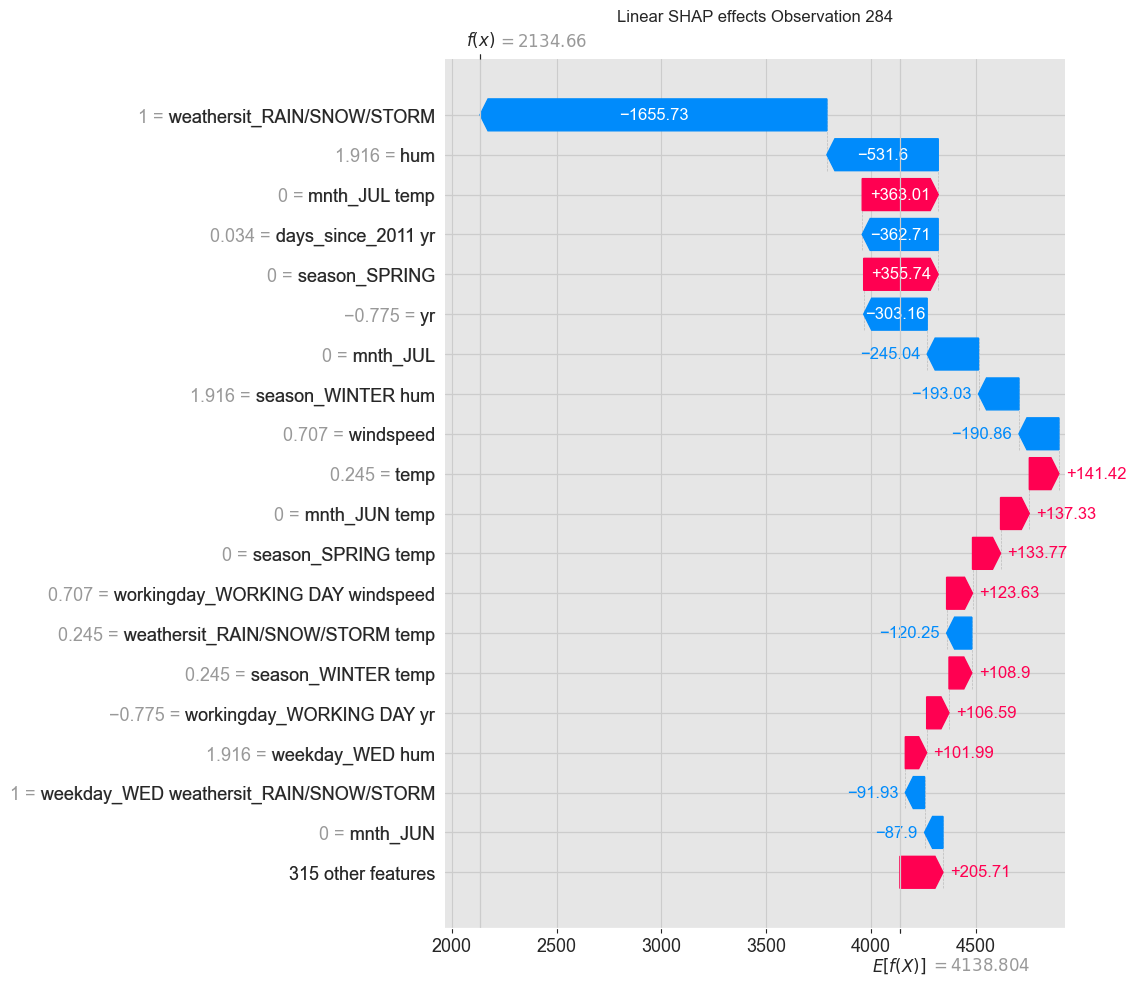
\includegraphics[scale=0.19]{images/interpretable_ml_122_0.png}
    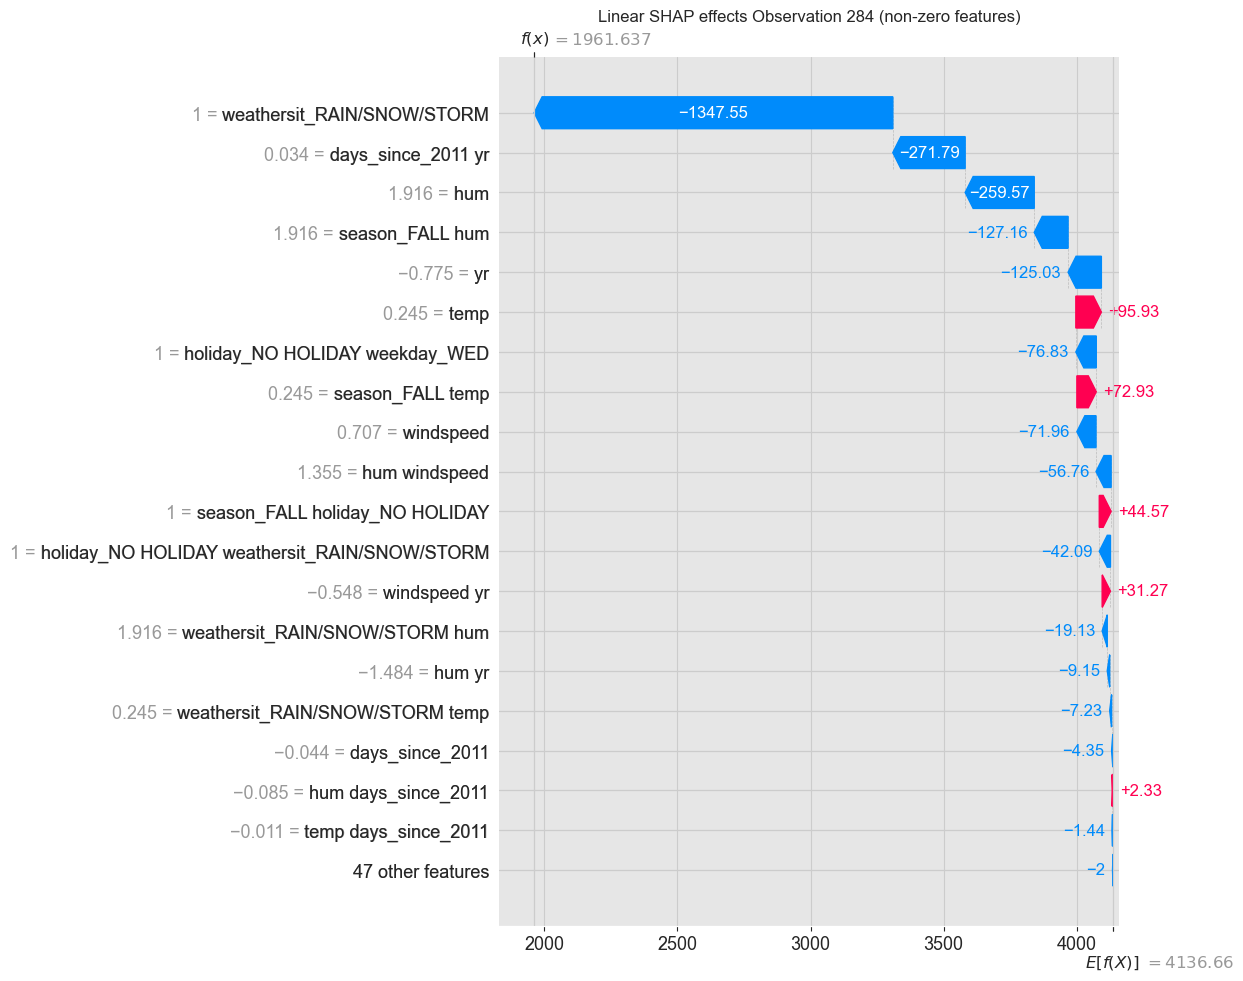
\includegraphics[scale=0.19]{images/interpretable_ml_134_0.png}
    \caption{This {\em waterfall plot} shows how the SHAP values of each feature move the model output from our prior expectation under the background data distribution, to the final model prediction given the evidence of all the features (\cite{NIPS2017_7062}). Compare with Figure \ref{fig:linear-284-obs}.}
  \end{figure}
\end{center}
\end{frame}


\section{References}

\begin{frame}[t, allowframebreaks]
\frametitle{References}
\footnotesize{
\setbeamertemplate{bibliography item}[text]
\bibliographystyle{plain}
\bibliography{references} 
}
\end{frame}

\begin{frame}
\begin{center}
\huge{Thank You!}
\end{center}

\begin{block}{Contact}
\begin{itemize}
\item \faRocket $\:$ \href{https://juanitorduz.github.io}{https://juanitorduz.github.io}
\item \faGithub $\:$ \href{https://github.com/juanitorduz}{github.com/juanitorduz}
\item \faTwitter $\:$ \href{https://twitter.com/juanitorduz}{juanitorduz}
\item \faEnvelope $\:$ \href{mailto:juanitorduz@gmail.com}{juanitorduz@gmail.com}
\end{itemize}
\end{block}

\begin{center}

\includegraphics[scale=0.08]{images/qr-code-juanitorduz.png} 
\end{center}

\end{frame}

\end{document}
